\section {Method and material}

We employed a hierarchical learning approach to classify the taxonomy of a virus based on its DNA sequence. Our method begins with an initial classifier that predicts the order of the virus. Once the order is identified, a second classifier is used to determine the family. Although further classifiers could be applied to predict the genus and species of the virus, this research focuses primarily on evaluating the effectiveness of the classifier. Therefore, we limited our study to the two viral orders, Martellivirales and Tymovirales.

After the order is predicted, the corresponding family classifier is applied to identify the specific family of the virus within that order. To maintain robust classification performance, we excluded families with fewer than five species and species with sequence lengths shorter than 100 base pairs.

This hierarchical approach enables accurate virus classification from DNA sequences, offering valuable insights into the virus’s characteristics and potential impact. By dividing the classification process into smaller, targeted steps, we effectively manage the complexity of viral taxonomy, enhancing our capacity to study and address viral threats.

In the following subsections, we discuss the dataset used, data preprocessing, and the machine learning model applied in this study.

\subsection{Dataset}
\label{sec:obj:det}

The dataset for this research was sourced from the National Center for Biotechnology Information (NCBI) RefSeq database, which offers high-quality, curated sequences that have been reviewed and annotated by experts, ensuring accuracy and reliability. RefSeq provides a single, well-characterized reference sequence for each virus, minimizing redundancy and simplifying data interpretation. Additionally, each RefSeq entry has a stable identifier, facilitating consistent referencing and reporting.

To acquire the relevant sequences, we used the latest Virus Metadata Resource (VMR) spreadsheet available from the International Committee on Taxonomy of Viruses (ICTV) at https://ictv.global/vmr/current, as well as on the associated GitHub repository. This file contains comprehensive metadata for all viruses. Using RefSeq accession numbers listed in the VMR spreadsheet, we downloaded the DNA sequences for the taxa of interest in this study.

In our research, we focused on the classification of viruses within the Alsuviricetes class, belonging to the Kitrinoviricota phylum, which is part of the Orthornavirae kingdom in the Orthornavirae realm. We developed a hierarchical classification approach, starting by categorizing viruses into two orders: Martellivirales and Tymovirales.

Subsequently, we employed specialized classifiers to distinguish among the families within each order. For the Martellivirales order, we differentiated between the families Virgaviridae, Closteroviridae, Bromoviridae, Togaviridae, Endornaviridae, and Solspiviridae. For the Tymovirales order, we further classified viruses into Betaflexiviridae, Alphaflexiviridae, and Tymoviridae families. This multi-level classification approach allowed us to systematically analyze and categorize the viral sequences with a high degree of precision. Table \ref{table:species_counts} provides an overview of the number of families and species in each order. This structured dataset enabled us to perform a comprehensive and precise classification of viral sequences across the chosen taxonomic levels.

\begin{table}[tb]
\centering
\begin{tabular}{| l | l | l |}
\hline
\textbf{Order} & \textbf{Family} & \textbf{Species} \\
\hline
\multirow{5}{*}{Martellivirales} & Virgaviridae & 56 \\
                                  & Closteroviridae & 54 \\
                                  & Bromoviridae & 38 \\
                                  & Togaviridae & 37 \\
                                  & Endornaviridae & 31 \\
\hline
\multirow{3}{*}{Tymovirales}     & Betaflexiviridae & 125 \\
                                  & Alphaflexiviridae & 65 \\
                                  & Tymoviridae & 34 \\
\hline
\end{tabular}
\caption{Number of families and species in each order.}
\label{table:species_counts}
\end{table}

\subsection{Hierarchical Classification}

\begin{figure*}[t]
\begin{centering}
		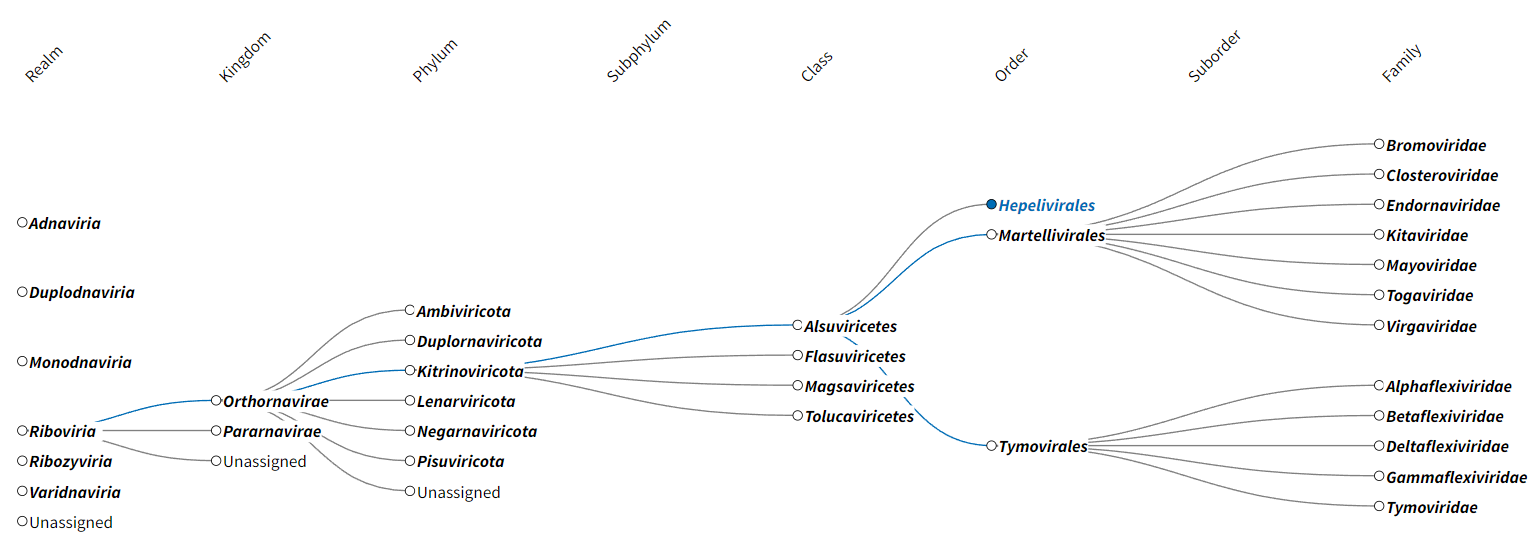
\includegraphics[width=\textwidth]{Figures/heirarchy_IVT.png}
	\caption{distribution  }
\label{fig:distr}
\end{centering}
\end{figure*}

The ICTV scheme organizes classes into a hierarchical taxonomic tree. From the highest to the deepest levels, these are: Realm, Kingdom, Phylum, Subphylum, Class, Order, Family, Subfamily, Genus, and Species. In hierarchical classification, our aim is to predict a set of hierarchically structured classes for each virus. A comprehensive review of hierarchical classification is available in [81][82]. Hierarchical classifiers can be categorized into three types based on how they utilize hierarchical information: the flat classifier approach, the local classifier approach, and the global classifier (big-bang) strategy. In this paper, we adopted the Local Classifiers per Parent Node (LCPN) approach. This approach reduces the number of classifiers compared to the Local Classifiers per Node (LCN) method, while still capturing hierarchical information. Unlike the flat classifier approach, LCPN explicitly incorporates the class hierarchy. Moreover, it is more intuitive and simpler than the big-bang classification strategy.

\begin{figure}[t]
\begin{centering}
		\includegraphics[width=.5\textwidth]{Figures/hierarchy2.png}
	\caption{distribution  }
\label{fig:distr}
\end{centering}
\end{figure}

\subsection{Classification Method}

In this paper, we implemented the Local Classifiers per Parent Node (LCPN) approach using a deep learning architecture. Specifically, we employed a 1D Convolutional Neural Network (CNN) to extract essential features from DNA sequences. These features were then passed to a Long Short-Term Memory (LSTM) layer, which captured sequential dependencies and patterns in the DNA data. The output from the LSTM layer was subsequently fed into a dense (fully connected) layer that was trained to accurately predict the class of the viral sequence.

\subsection{Data Preprocessing} To ensure the quality and consistency of our dataset, we implemented several sequence pre-processing steps. First, we excluded viral families with fewer than five sequences, as well as any sequences shorter than 100 nucleic acids. This filtering step reduced noise and ensured that our dataset had sufficient representation across families. The final distribution of families and the number of species in each family is depicted in Figure~\ref{fig:distr}.


Next, we addressed the issue of unidentified nucleic acids. For DNA sequences, any character that was not A, T, G, or C was replaced with the most frequent nucleic acid in that sequence. Similarly, for RNA sequences, we replaced characters that were not A, U, G, or C with the most frequent nucleic acid. This step minimized the impact of ambiguous nucleotides and improved the quality of the input data for subsequent analysis.

We applied two data augmentation schemes to increase the size of our training dataset. The first scheme involves generating the reverse complement of each DNA sequence. The reverse complement is obtained by reversing the order of nucleotides in the original sequence and replacing each nucleotide with its complementary base pair (A with T, T with A, C with G, and G with C). For example, the reverse complement of the sequence ATCG is CGAT.

This augmentation strategy effectively doubles the amount of training data while preserving the biological significance of the sequences. By including both the original and reverse complement sequences, we ensure that the model learns to recognize patterns regardless of sequence orientation, thereby enhancing its robustness and accuracy without introducing any bias or sacrificing performance.

Next, we encoded the nucleotides using one-hot encoding instead of the more commonly used k-mer encoding. One-hot encoding offers the advantage of preserving the sequential information of each nucleotide, allowing the model to learn fine-grained patterns in the DNA sequence. Unlike k-mer encoding, which abstracts sequences into overlapping k-length subsequences and may lose positional details, one-hot encoding ensures that each nucleotide's unique position is explicitly represented. This encoding method is particularly effective for models such as 1D CNNs and LSTMs, which rely on precise sequential and spatial information to capture important biological features

Our second approach involves splitting each sequence (and its reverse complement) into $m$ subsequences of length $n$ using a sliding window with a stride $s$. To ensure uniformity across the dataset, we dynamically adjust the stride $s$ for each sequence so that all sequences generate the same number of subsequences of equal length. The stride $s$ is calculated using the formula:
$$  s = \frac{L-n} {m-1},$$

 
where $L$ is the total length of the sequence, $n$ is the length of each subsequence, 
$m$ is the number of subsequences to generate, and $s$ is the step size for the sliding window, which determines how far the window moves between generating subsequences. For example, to generate 3 subsequences, each of length 100, from a sequence of length 300, the stride would be 100. In contrast, to generate 3 subsequences of length 100 from a sequence of length 200, the stride would be 50.

This method ensures that all sequences contribute equally to the training process, regardless of their original length, thereby enhancing the robustness and generalizability of the model. By maintaining consistent input dimensions, we minimize the risk of overfitting to specific sequence lengths and ensure that our model can effectively learn patterns across the entire dataset. Additionally, incorporating both the original and reverse complement sequences helps capture relevant features that may be orientation-dependent, further strengthening the model’s ability to generalize to unseen data
 
\neuralnetwork{
  layers={ 3, 4, 2 },
  labels={ {Input Layer}, {Hidden Layer}, {Output Layer} }
}



